\subsection{Zastosowanie .NET MAUI}

.NET MAUI pozwala na użycie logiki programu na różnych platformach 
(w przypadku mojej pracy Android oraz Windows).
Każdy element interfejsu jest stworzony i wyświetlany zgodnie z natywnymi elementami, 
które są oferowane przez daną platformę. Takie podejście pozwala na skorzystanie 
z ewentualnych optymalizacji oferowanych przez twórców danego systemu oraz 
zachowanie jednolitego wyglądu aplikacji ze środowiskiem.

W .NET MAUI widoki możemy tworzyć na dwa sposoby - albo dynamicznie w plikach C\# \verb|.cs|, 
albo w plikach \verb|.XAML|. W mojej pracy zdecydowałem się na skorzystanie z tej drugiej opcji 
ze względu na wyższą wydajność aplikacji~\cite{xamlPerformance} oraz sposób ich definiowania 
(korzystając ze wzorca MVVM dobrze jest podzielić kod między różne pliki, 
a przy zastosowania XAMLa odbywa się to naturalnie).

\verb|XAML| to akronim od E\textbf{x}tensble \textbf{A}pplication \textbf{M}arkup \textbf{L}anguage, 
czyli rozszerzalnego języka znaczników aplikacji. Pozwala na uporządkowane i wyczerpujące opisanie 
widoków aplikacji, podpięcia (ang. Binding) wartości o róznych typach pod określone właściwości 
elementów, co pozwala na dynamiczne zmienianie parametrów każdej z części interfejsu użytkownika - 
począwszy od widoczności, kolorów, umiejscowienia, aż po zaimportowanie danych i dynamiczne generowanie 
powtarzalnych fragmentów (dobrym przykładem będzie kontrolka \verb|CollectionView|).
Jego struktura wywodzi się z XML, który jest optymalnym kompromisem pomiędzy czytelnością kodu dla człowieka 
oraz przewidywalnością i kompletnością składni dla komputera.

Na rysunku \ref{img:mauiArchitectureDiagram} możemy zaobserwować, jak kod aplikacji 
zostaje za pomocą .NET MAUI przekonwertowany na różne systemy operacyjne (3 rząd), 
a następnie ponownie przetłumaczony na elementy zdefiniowane w .NET BCL, 
czyli Base Class Library (biblioteki klas bazowych). \\
\begin{figure}[hb]
    \centering
    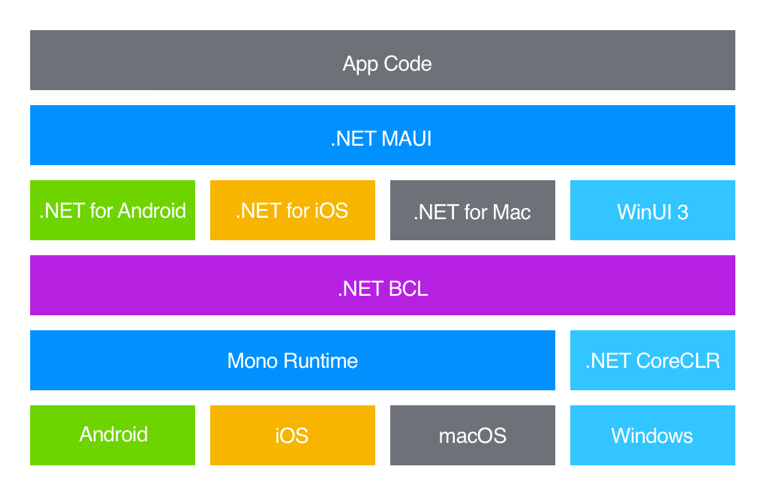
\includegraphics[width=\textwidth]{mauiArchitectureDiagram.png}
    \caption{Diagram architektury .NET MAUI wśród wszystkich obsługiwanych platform~\cite{mauiDefinition}}
    \label{img:mauiArchitectureDiagram}
\end{figure}
